Due to the aforementioned notable differences between the two architectures, executing an x86-64 binary on a RISC-V system is not a trivial task. We will now lay out the main challenges that arise, discuss possible solutions, and explain core concepts.

\subsection{Scope Definition}
The purpose of oxtra is to execute programs compiled for x86-64 on a RISC-V system. We do not aim for completeness, especially since many of the x86-64 instructions are already deprecated. Instead, our goal is to support a subset of x86-64 that allows execution of small, statically linked command line programs such as gzip\footnote{\url{https://www.gzip.org} (visited on 13/10/2019)}. In particular, SSE instructions (and by extension the use of floating-point numbers) and threading are not supported in the initial release of oxtra. Neither of these are natively supported by the RISC-V ISA (at time of writing) and their implementation would be far more complex than the scope of this project allows for. A complete list of supported instructions can be found in Appendix \ref{Supported Instructions}.
By focusing our attention, we are able to keep our project lightweight and aim to outperform our competitors.

\subsection{Binary Translation}
	The wording Binary Translation already perfectly describes itself. Translating one executable binary object into another executable binary object. In the case of oxtra, this means translating a language written for the x86-64 processor into a language understandable by a processor of the RISC-V family. 

	\subsubsection{Core Principles}
		Every approach to binary translation requires three major components in one or the other shape and form. The first component (i.e. step) consists of decoding: the source language has to be decoded into a data structure understandable by the translation process. The second step remaps the data structure into a format, which can be implemented on the destination architecture. The third component is the encoding of the data structure into the destination language. Some approaches to binary translation warp these components or decrease them to near zero, but some aspects of them can always be found.
		Binary Translation itself enrolls into a set of different projects and approaches. The most noteworthy are emulation, static translation, and dynamic translation:

	\paragraph{Emulation}
		is the process of executing a binary by interpretation without generating a new binary. The main advantage of emulation is the ability to write the translation unit without having to accommodate any specific host architecture, although this comes at a significant loss of performance.

	\paragraph{Static Translation}
		systems (also called full translation systems) transform a source binary into a new binary that replicates the behavior of the source binary. Full translation allows for analyzing the source and optimizing the generated binary, yielding very fast host code at the cost of significant up-front overhead. However, since the source is never executed, some aspects such as evaluating indirect jumps become a very difficult task and may even require manual labor.

	\paragraph{Dynamic Translation}
		can be considered as a combination of the previous two methods. The generation of a new binary is done in small chunks that are immediately executed after translation. Even though this does not allow for much optimization since the control flow cannot be known without preprocessing, it is still often faster than emulation since there is less overhead. The generated code is usually not written to long-term storage.
	
	\subsubsection{Oxtra as a dynamic Translator}
		Oxtra is a dynamic binary translator. The three core components of a binary translator can be distinctly separated with our design. Oxtra loads a source binary and translates parts of the binary on demand, without processing the binary further. Those translated code chunks, are optimized as well as possible within themselves. Due to the lack of control path analysis, the instructions of a chunk cannot be merged with each other, as future code might require jumping right into two otherwise merged instructions, which could lead to undefined behavior.

% Binary Translation in general
% Vorteil einer Intermediate Language
% Vorteil von direktem Übersetzen
% Was sind grundsätzlich die Problem bei sowas
% Vielleicht die Infographik von Knud Just In Time Compilation
% Notwendigkeit eines Decoders und Encoders (Kernkomponenten)
% Unterschied Just in Time, Emulation, Komplette Translation (File->File), was sollte man machen
% Welche Optimierungen sind möglich (Branch Prediction, Loop unrolling ...)

\subsection{Unit of Translation}
\label{blocks}
	When using dynamic binary translation, the executable has to be split into smaller chunks with multiple instructions, so-called \emph{blocks}, that can be translated at once. The maximum number of instructions per block has a significant impact on the performance of the overall translation process. A rather small maximum block size can result in a substantial performance overhead caused by many non-sequential instructions (i.e. jumps to the translator). Too large blocks on the other hand can lead to wasting time on instructions that may never be executed. As a basic unit of translation, many DBTs split instructions into basic blocks \cite{qemu-conference-paper, arm-binary-translator}.

	\subsubsection{Basic Blocks} % Basic blocks, linking
		A basic block is a group of linear instructions with a well-defined single point of exit at the end. Each instruction that changes the control flow (e.g. jump) marks the end of such a basic block. The operations making up a basic block can be viewed as a \emph{single}, sophisticated instruction\footnote{This interpretation does not always hold true, especially with exception handling. For example, with every memory access an exception could be triggered, causing the basic block to have another (partially undefined) exit.} that can be executed linearly without modification of the execution flow. This absoluteness of basic blocks makes them the ideal candidate for the core chunk size used in the translation process. \autoref{fig:basicblocks} illustrates how code is separated into two basic blocks. 

		\begin{figure}[htb]
			\begin{subfigure}[b]{.5\textwidth}
				\centering
				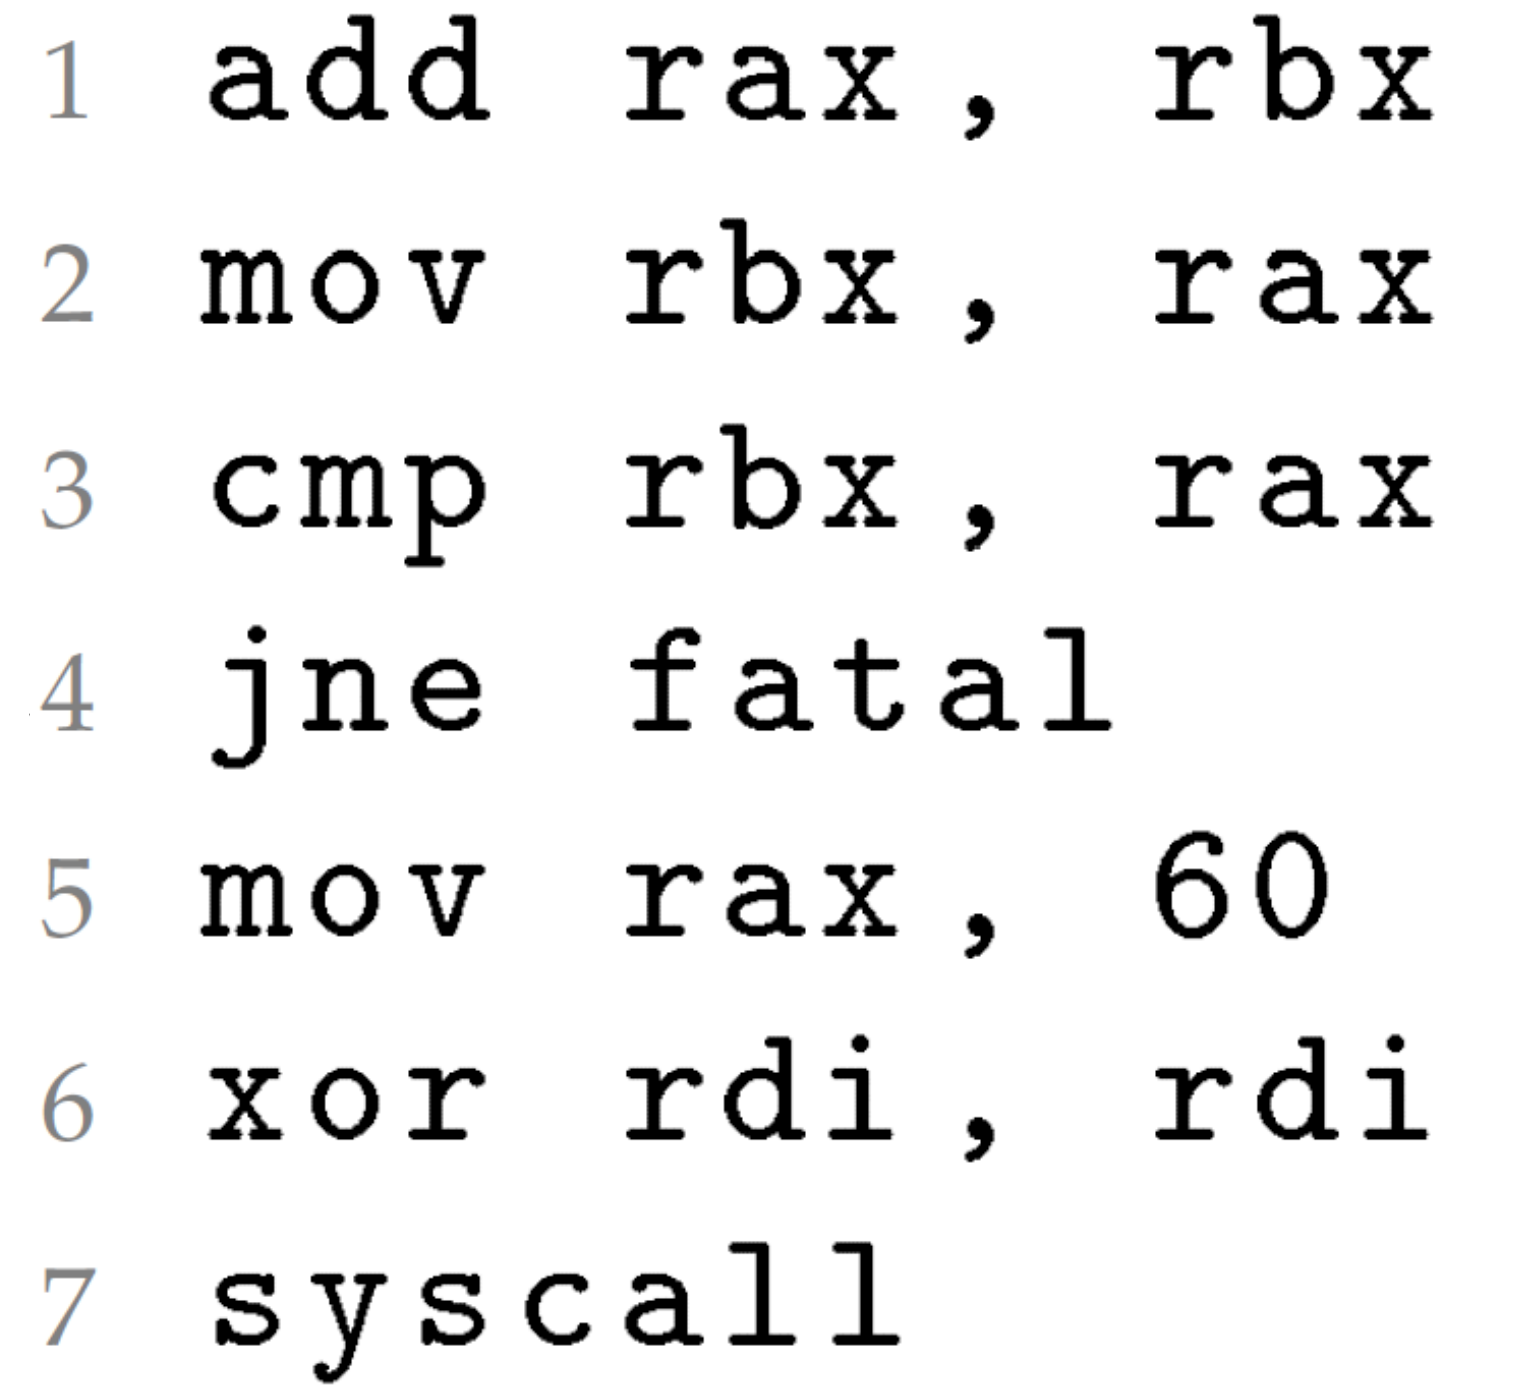
\includegraphics[width=0.4\linewidth]{basic_block}
				\caption{Before Basic Block Creation}
				\label{fig:basicblocks-before}
			\end{subfigure}
			\begin{subfigure}[b]{.5\textwidth}
				\centering
				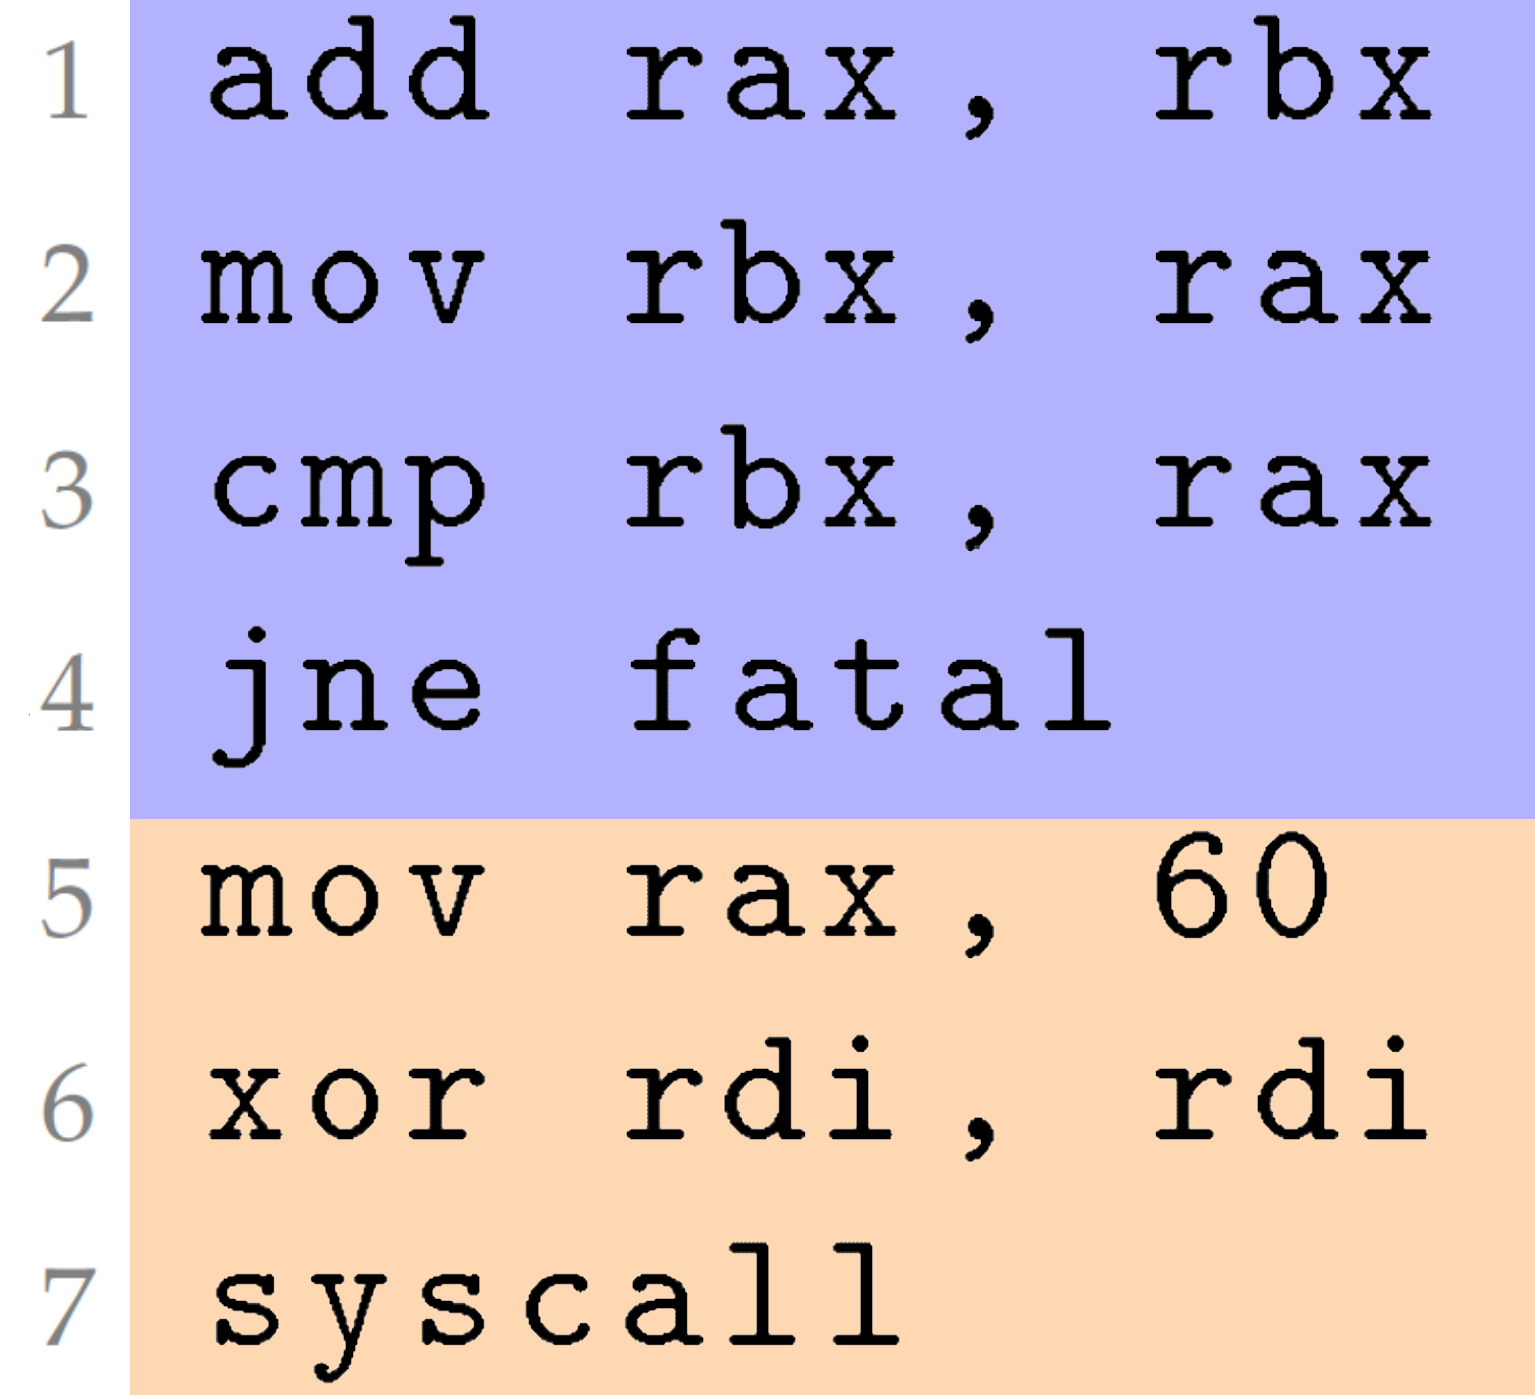
\includegraphics[width=0.4\linewidth]{basic_block_colored}
				\caption{After Basic Block Creation}
				\label{fig:basicblocks-after}
			\end{subfigure}

			\caption[Basic Block Separation]{An example on the scope of basic blocks (in x86-64 assembly).}
			\label{fig:basicblocks}
		\end{figure}

		The final instruction of every basic block can be understood as a link, or a reference to another block (or the end of execution). With this interpretation of links, each executable can be depicted as a set of multiple basic blocks linked with each other. Those links can either be \emph{static}  or \emph{dynamic}. Static links have a constant target, such as a direct jump to an address (e.g. \texttt{jmp label}). Whereas dynamic links have a variable target, for example an indirect jump (e.g. \texttt{jmp rax}).
		
	\subsubsection{Linking Blocks}
	\label{Block Chaining}
		Since the actual target (i.e. the address of the executable RISC-V code) is (initially) unknown, the destination has to be evaluated at runtime by the host. The first time a static link is accessed, the host evaluates the target address once and modifies the link so that it points directly to an instruction in a block. \emph{Block Chaining} describes this concept of permanently connecting two statically linked blocks by evaluating the destination only once at translation time.
	
		Dynamic links on the other hand are always indirect: Since the target depends on an external, unknown value (e.g. a register), the target of the link can only be determined by the host. This means, that the address has to be evaluated every time the link is taken.
		
		Chaining blocks may drastically save time in hot paths since the translator only has to be called once. Additionally, this allows for the execution of multiple basic blocks at once, without further intervention of the host.
		
	\subsubsection{Super Blocks}
	Basic blocks with multiple exit points and as single entry are called \emph{super blocks}. With these, conditional jumps do not necessarily have to end the block, allowing the execution of more code without intervention of the host. If two super blocks reference the same basic block, it may be better to duplicate the generated code instead of adding additional jumps \cite{smith2005virtual}. With duplicated code, both super blocks can be larger and function independently.

\subsection{Code Storage}
\label{code storage}
After a block of code has been translated, it must be decided how long it should be stored. Many programs run sequentially, meaning that except for loops it is rare for already executed parts to be revisited. One option for storing translated code is to implement a so-called code cache. By deleting older sections of translated code on the assumption that they will not be executed again, a DBT can save a lot of memory depending on the size of the guest program.

When storing translated code indefinitely on the other hand, the target of a jump is consistent, as the addresses of instructions are permanent. Since the code translation process itself causes some overhead, a permanent code storage may drastically reduce the number of translations. The reallocation of already translated code has to be handled with special care in this configuration, as all jumps to already translated blocks become invalid.

Another situation the code store must handle is a jump to an arbitrary instruction of a basic block instead of the beginning. This poses no problem if blocks are stored in a way that allows access to the addresses of individual translated instructions\footnote{This is not entirely trivial since a single x86-64 instruction may be translated into multiple RISC-V instructions.}. If, however, this is the first time that the basic block is accessed, it has to be translated first, meaning that the part before the jump target will be left untranslated. If the guest ever tries to access that part, the DBT will have to either re-translate the whole block and store it twice, relocate the already translated part to join it with the new part (and fix any jumps that target that block), or add a jump to the old part at the end of the new one.

\subsection{Execution}
Executing the guest program concurrently with the host is a rather complex process. Since guest and host could interfere with each other, countermeasures have to be taken to separate the two programs. Fully hiding the host from the guest is not feasible since this would cause a lot of performance overhead. The aim is to run the guest and host in parallel without issues during execution. 

	\subsubsection{Context Differentiation}
	\label{context}
		% Different registers
		% Different stacks
		Unlike in emulation where the guest program is always completely encapsulated by the emulator, a program executed by dynamic binary translation takes full control of the CPU. It will not only change values in registers and memory but also expect these changes to persist between jumps. Unless the host architecture has an absolute abundance of registers to the point where the register space can be split between guest and host (and usually it does not), this necessitates the DBT to keep track of the guest state; store it when the guest reaches a dynamic link, and restore it once execution can continue.
		
		Another essential part is the stack. Unlike registers, this resource could be shared between guest and host by letting the guest operate on the lower half of the host's stack, but this would allow the guest to potentially invalidate the host's stack (e.g. cause a stack overflow). For this reason, it is usually a good idea to allocate a separate stack for the guest.
		
		The combination of those two parts, the stack and all registers, make up the \emph{context}. Guest and host each have their own context that has to be kept track of during the execution process.
		
	\subsubsection{Register Mapping}
	\label{register_mapping}
		Since the guest program expects to be able to access any register, the DBT has to map the space of guest registers to the space of host registers and/or emulate them in memory. Fortunately, RISC-V provides more general-purpose registers than x86-64 (ignoring SSE\dots), which allows every x86-64 register to be mapped to a RISC-V register while still leaving some registers unmapped. These unmapped registers are quite important since the translation of complex instructions often requires storing intermediate values. A few registers could even be used to store a pointer to important jump targets, such as the function for context switching.
		
	\subsubsection{Memory Layout}
		% Grundproblem, dass wir zwei verschiedene Speicherebereiche brauchen
		% Mögliche Lösungen: Memory emulieren, oder yolo auf hohe Adresse linken (yolo, weil man Memory-Konflikte mit uns bekommen soll)
		One could create a second process for the guest application, allowing guest and host to exist side by side with two different address spaces. However, this would require not one, but two context switches to transfer control between the guest and the DBT (guest \(\rightarrow\) OS \(\rightarrow\) DBT), which is one of the most expensive operations in dynamic binary translation.
		
		Another approach is to realize that since the guest program is effectively part of the DBT, it can share an address space with it. If the host platform has a larger address space than the guest, one can simply use the addresses not available on the guest platform for the DBT without fear of interference from the guest. If both platforms have the same address space however, memory conflicts could arise.
		
		One method of solving this conundrum is to emulate the guest memory. However, one could run into difficulties if the guest platform has smaller page sizes than the host and (for memory efficiency) multiple guest pages are mapped to the same host page. This becomes problematic if the guest tries to give those pages different memory protection modes. To solve this problem the DBT could decide to be very lenient and give each of the pages the most allowing of the requested protection modes, which can obviously cause problems if the guest is not well behaved. In that case, the only solutions are to either give each page the most restrictive of the requested protection modes, necessitating the DBT to potentially emulate every memory access (slow), or to give each guest page its own host page, which not only requires a lot more memory but also means that the guest's address space is no longer continuous.
		
		A simpler method would be to figure out which part of the address space usually goes unused on the guest platform and map the DBT to those addresses\footnote{If an application relies on this specific address space, it cannot be executed by the DBT without further modification of either the DBT itself or the host application.}. If one was concerned with safety, one could write-protect those pages and start emulating memory if the guest tries to access them.

	\subsubsection{Dynamic Translation}
		% Sprung zu unserem Programm und wieder zurück
		% Context speichern
		% Dispatcher
		In order to allow for the execution of two programs side by side, a mechanism has to be put into place that specifies when and how to switch between them. In a DBT this role is usually taken up by a so-called \emph{dispatcher}.
		
		The basic idea is that if the guest program encounters an operation that interrupts the execution flow, i.e. a link, the guest context will be saved, and the dispatcher is called. The task of the dispatcher is to ensure that execution of the guest can continue. For this purpose, it may just load the address of the requested jump, or it may have to call out to a system call handler or a translator. Once all the necessary steps have been taken, the guest context will be restored, and guest execution may resume.

\subsection{Control Flow}
	Control flow instructions (such as jumps/calls) mark the end of a basic block and may require costly operations like dynamic block linking or flag evaluation.
	
	\subsubsection{Flags}
		\label{approach_flags}
		% nicht wie es bei uns implementiert ist, sondern dass es einen großen Unterschried bei Sprüngen etc gibt.
		% eager (egal bei HW support) / lazy (gut für RISC-V) evaluation Vergleich
		One of the bigger differences between the two architectures of interest to this project is the handling of conditional branching. The way x86-64, along with most other popular architectures \cite{arm, ppc}, implements it is by having a register dedicated to storing information about the result of the last arithmetic operation. RISC-V on the other hand does not store any information about previous (integer) operations, opting to use fused compare-and-branch instructions instead\footnote{RISC-V does have a flags register for floating point operations}.
		
		The obvious solution would be to emulate the x86-64 behavior, meaning that the DBT must manually update a dedicated flags register after every arithmetic operation, so called \enquote{eager} evaluation. Unless there is hardware support, evaluating flags can be quite costly, especially more complex ones like parity. A more efficient albeit less accurate method is to evaluate flags only for the last arithmetic operation(s) before the flags register is read (e.g. before a conditional jump), so called \enquote{lazy} evaluation. Since flags are often set and then immediately discarded, lazy evaluation can save a lot of time while still being transparent to the guest program. The difference between eager and lazy evaluation is illustrated in \autoref{fig:flageval}.
		
		\begin{figure}[htb]
			\centering
			\begin{subfigure}[b]{.5\textwidth}
				\centering
				\begin{lstlisting}[frame=none,xleftmargin=2.7cm]
add rax, rbx
update flags
add rax, rcx
update flags
add rax, rdx
update flags
jcc label
				\end{lstlisting}
				\caption{Eager Flag Evaluation}
				\label{fig:flageval-eager}
			\end{subfigure}%
			\begin{subfigure}[b]{.5\textwidth}
				\centering
				\begin{lstlisting}[frame=none,xleftmargin=2.7cm]
add rax, rbx
add rax, rcx
add rax, rdx
update flags
jcc label
				\end{lstlisting}
				\caption{Lazy Flag Evaluation}
				\label{fig:flageval-lazy}
			\end{subfigure}
			\caption{Comparison of eager and lazy flag evaluation.}
			\label{fig:flageval}
		\end{figure}

	\subsubsection{Jump}
	\label{translating conditional jumps}
	% Flag support wird da benötigt
	% Adresse dynamisch berechnen bei Sprung zu Register -> Sprung zu Programm (z.B.:)
	Since branching instructions could target not yet translated sections of code, they cannot be translated directly but instead a jump to the dispatcher will be generated. Once there, the dispatcher can examine the target and request translation of it if necessary. If the jump is static, the dispatcher may then replace the call to itself with a jump to the (critically) unchanging actual target (see \autoref{fig:jumptranslation}). This context switch can be eliminated by implementing block chaining (see \ref{Block Chaining}). However, if the jump is dynamic, the dispatcher will have to be called every time to ensure the target is translated and executable.
	
	Note that since the following block could depend on flags set in the current block, all flags have to be updated (even for unconditional jumps). The translation unit can use a look-ahead that recursively analysis following blocks to eliminate many of those unnecessary flag updates. This look-ahead is especially useful with x86-64, as most flags are discarded.
	
	\begin{figure}[htb]
	\centering
	\begin{subfigure}[b]{0.33\textwidth}
		\centering
		\begin{lstlisting}[frame=none,xleftmargin=1.3cm]
jmp label
		\end{lstlisting}
		\caption{x86 Input Code}
		\label{fig:jumptranslation-x86in}
	\end{subfigure}%
	\begin{subfigure}[b]{.33\textwidth}
		\centering
		\begin{lstlisting}[frame=none,xleftmargin=1.1cm]
nop
jalr 0, s11, 0
		\end{lstlisting}
		\caption{Initial Translation}
		\label{fig:jumptranslation-beforedispatcher}
	\end{subfigure}
	\begin{subfigure}[b]{.33\textwidth}
		\centering
		\begin{lstlisting}[frame=none,xleftmargin=0.7cm]
addi t0, zero, label
jalr 0, t0, 0	
		\end{lstlisting}
		\caption{Final Translation Result}
		\label{fig:jumptranslation-afterdispatcher}
	\end{subfigure}
	\caption{Process of translating a static jump (\texttt{s11} stores a pointer to the dispatcher).}
	\label{fig:jumptranslation}
\end{figure}
	
	\subsubsection{Call and Return}
		The x86-64 \texttt{call} instruction pushes the return address (the address of the instruction following the call) onto the stack and then jumps to the address specified in the \texttt{call}. The \texttt{ret} instruction pops the return address from the stack and jumps to it. The naive approach to translating these is by translating the \texttt{call} as a push of the return address and a jump to the specified address. A \texttt{ret} would pop the return address and look for the RISC-V code in the code store or translate it, if it's not cached. However, the lookup in the code store is costly and would have to be performed for each execution of \texttt{ret}. Fortunately, there are ways to resolve this issue. 
		
		One of them is to alter the behavior of the \texttt{call} such that it translates the basic block starting from the return address and pushes the address of the generated RISC-V code. \texttt{ret} could then just pop that address and jump to it directly. This approach is fine for most C programs, because they neither read nor modify the return address, but results in undefined behavior if the program relies on such techniques. It also requires storing the translated code indefinitely.
		
		A second option would be to implement a return stack similar to what many modern processors use for branch prediction \cite{arm-technical-reference-manual}. The return stack holds information that is used by \texttt{ret} in two ways:
		\begin{enumerate}
			\item Check if the return address has been altered. In this case \texttt{ret} has to find the code that corresponds to the new return address dynamically.
			\item Find the RISC-V code of the original, unmodified return address efficiently.
		\end{enumerate}
		This information is provided by \texttt{call}, which does not only push the return address onto the guest stack but also additional information onto the return stack.
		
	\subsubsection{System Calls}
	\label{approach_syscalls}
		% Exit Syscall "problematisch"
		% nicht reines durchgeben
		% Indizes der Syscalls verändern sich
		% Syscall könnten theoretisch unseren Heap zerstören (bei z.B. remapping, brk)
		Communicating with the operating system/kernel is an essential operation, but the interface greatly differs between architectures. While a special \emph{syscall} instruction may be a constant, the system call index, the expected arguments or even the existence of such a system call is far from invariant. For example, the \texttt{open} system call (index 2), which is supported in x86-64, has been replaced by \texttt{openat} (index 56) in RISC-V; numbering also differs.
	
		Additionally, some system calls could have highly destructive effects on the DBT, for example \texttt{exit}, which would not allow the DBT to clean up after itself, or \texttt{brk}, which could destroy the DBT's memory. As such, the DBT needs to intercept any system calls and emulate them appropriately, effectively acting as the operating system as far as the guest is concerned.
	
\subsection{ELF}
	The Executable and Linkable Format (ELF) is a file format used by Linux and Unix like systems to distribute binaries and dynamically linked libraries. Even though the ELF format is not originally from Linux, most binaries nowadays produced on modern Linux systems will come in the form of an ELF file. An ELF file contains everything required to run the included binary. This includes various information about the required environment (e.g. architecture, stack size) as well as the binary itself and data required by the binary. To execute an ELF binary, the file only needs to be loaded partially into memory. 
	
	\subsubsection{Sections} 
	The core principle of the ELF format is the concept of sections. Sections are primarily used in the linking process to link multiple ELF files together. A single ELF file can contain many sections. A section consists of a name, a virtual address and size, which describe where the section should reside in memory once the ELF file is loaded. It also contains a file offset and file size which describe where the data reside within the file. Additionally, it contains attributes which describe whether the contents should be flagged as readable, writable, and/or executable or whether the section contains any information in the file, and if it should be loaded into memory in the first place.
	
	There are some default names (e.g. \texttt{.text}, \texttt{.bss}, \texttt{.symtab}) of which the sections are expected to hold the information described by their name. By default, the text section contains the executable code and the bss section should contain uninitialized data (it is flagged as containing no data in the file, and only in memory). The symtab section contains a list of symbols defined by the binary. A symbol is a pair of a name (e.g. function name or variable name) and an address, which describes where to find it. But every compiler can add as many sections as required.
	
	\subsubsection{Program Headers}
	The ELF format also describes the program header: every ELF file contains a list of program headers. They simplify the work of loading the binary into memory when trying to execute it. Every program header contains virtual address and size information, as well as file offset information. The program headers are used for executing a binary: when the program headers have been loaded into memory it is ensured that all necessary data required to run the binary are in the memory. The program header also contains necessary information required to potentially load shared libraries and to dynamically link the binary to these. 
	
	\subsubsection{Shared Libraries}
	Most ELF files do not contain all the code required to run the binary or all the data required. This is because code and data might be shared between multiple binaries. Thus, they have to be dynamically linked for the initial binary to work properly. The program header list in the ELF file contains entries, which hold the name of required ELF file(s) as well as the name of the interpreter required. The interpreter processes the information about the dynamic linking and handles the entire linking process. Those required binaries might also depend on (possible multiple) other ELF files. For the program to be executed properly, all these requirements have to be satisfied. In order to link those ELF files, the program headers are required, as they contain special entries. These entries tell the interpreter, where the addresses of other ELF files and some of their symbols have to be written to.